\documentclass[ignorenonframetext,]{beamer}
\setbeamertemplate{caption}[numbered]
\setbeamertemplate{caption label separator}{: }
\setbeamercolor{caption name}{fg=normal text.fg}
\beamertemplatenavigationsymbolsempty
\usepackage{lmodern}
\usepackage{amssymb,amsmath}
\usepackage{ifxetex,ifluatex}
\usepackage{fixltx2e} % provides \textsubscript
\ifnum 0\ifxetex 1\fi\ifluatex 1\fi=0 % if pdftex
  \usepackage[T1]{fontenc}
  \usepackage[utf8]{inputenc}
\else % if luatex or xelatex
  \ifxetex
    \usepackage{mathspec}
  \else
    \usepackage{fontspec}
  \fi
  \defaultfontfeatures{Ligatures=TeX,Scale=MatchLowercase}
\fi
% use upquote if available, for straight quotes in verbatim environments
\IfFileExists{upquote.sty}{\usepackage{upquote}}{}
% use microtype if available
\IfFileExists{microtype.sty}{%
\usepackage{microtype}
\UseMicrotypeSet[protrusion]{basicmath} % disable protrusion for tt fonts
}{}
\newif\ifbibliography
\hypersetup{
            pdftitle={Random Effects ANOVA},
            pdfborder={0 0 0},
            breaklinks=true}
\urlstyle{same}  % don't use monospace font for urls
\usepackage{color}
\usepackage{fancyvrb}
\newcommand{\VerbBar}{|}
\newcommand{\VERB}{\Verb[commandchars=\\\{\}]}
\DefineVerbatimEnvironment{Highlighting}{Verbatim}{commandchars=\\\{\}}
% Add ',fontsize=\small' for more characters per line
\usepackage{framed}
\definecolor{shadecolor}{RGB}{248,248,248}
\newenvironment{Shaded}{\begin{snugshade}}{\end{snugshade}}
\newcommand{\KeywordTok}[1]{\textcolor[rgb]{0.13,0.29,0.53}{\textbf{#1}}}
\newcommand{\DataTypeTok}[1]{\textcolor[rgb]{0.13,0.29,0.53}{#1}}
\newcommand{\DecValTok}[1]{\textcolor[rgb]{0.00,0.00,0.81}{#1}}
\newcommand{\BaseNTok}[1]{\textcolor[rgb]{0.00,0.00,0.81}{#1}}
\newcommand{\FloatTok}[1]{\textcolor[rgb]{0.00,0.00,0.81}{#1}}
\newcommand{\ConstantTok}[1]{\textcolor[rgb]{0.00,0.00,0.00}{#1}}
\newcommand{\CharTok}[1]{\textcolor[rgb]{0.31,0.60,0.02}{#1}}
\newcommand{\SpecialCharTok}[1]{\textcolor[rgb]{0.00,0.00,0.00}{#1}}
\newcommand{\StringTok}[1]{\textcolor[rgb]{0.31,0.60,0.02}{#1}}
\newcommand{\VerbatimStringTok}[1]{\textcolor[rgb]{0.31,0.60,0.02}{#1}}
\newcommand{\SpecialStringTok}[1]{\textcolor[rgb]{0.31,0.60,0.02}{#1}}
\newcommand{\ImportTok}[1]{#1}
\newcommand{\CommentTok}[1]{\textcolor[rgb]{0.56,0.35,0.01}{\textit{#1}}}
\newcommand{\DocumentationTok}[1]{\textcolor[rgb]{0.56,0.35,0.01}{\textbf{\textit{#1}}}}
\newcommand{\AnnotationTok}[1]{\textcolor[rgb]{0.56,0.35,0.01}{\textbf{\textit{#1}}}}
\newcommand{\CommentVarTok}[1]{\textcolor[rgb]{0.56,0.35,0.01}{\textbf{\textit{#1}}}}
\newcommand{\OtherTok}[1]{\textcolor[rgb]{0.56,0.35,0.01}{#1}}
\newcommand{\FunctionTok}[1]{\textcolor[rgb]{0.00,0.00,0.00}{#1}}
\newcommand{\VariableTok}[1]{\textcolor[rgb]{0.00,0.00,0.00}{#1}}
\newcommand{\ControlFlowTok}[1]{\textcolor[rgb]{0.13,0.29,0.53}{\textbf{#1}}}
\newcommand{\OperatorTok}[1]{\textcolor[rgb]{0.81,0.36,0.00}{\textbf{#1}}}
\newcommand{\BuiltInTok}[1]{#1}
\newcommand{\ExtensionTok}[1]{#1}
\newcommand{\PreprocessorTok}[1]{\textcolor[rgb]{0.56,0.35,0.01}{\textit{#1}}}
\newcommand{\AttributeTok}[1]{\textcolor[rgb]{0.77,0.63,0.00}{#1}}
\newcommand{\RegionMarkerTok}[1]{#1}
\newcommand{\InformationTok}[1]{\textcolor[rgb]{0.56,0.35,0.01}{\textbf{\textit{#1}}}}
\newcommand{\WarningTok}[1]{\textcolor[rgb]{0.56,0.35,0.01}{\textbf{\textit{#1}}}}
\newcommand{\AlertTok}[1]{\textcolor[rgb]{0.94,0.16,0.16}{#1}}
\newcommand{\ErrorTok}[1]{\textcolor[rgb]{0.64,0.00,0.00}{\textbf{#1}}}
\newcommand{\NormalTok}[1]{#1}
\usepackage{longtable,booktabs}
\usepackage{caption}
% These lines are needed to make table captions work with longtable:
\makeatletter
\def\fnum@table{\tablename~\thetable}
\makeatother
\usepackage{graphicx,grffile}
\makeatletter
\def\maxwidth{\ifdim\Gin@nat@width>\linewidth\linewidth\else\Gin@nat@width\fi}
\def\maxheight{\ifdim\Gin@nat@height>\textheight0.8\textheight\else\Gin@nat@height\fi}
\makeatother
% Scale images if necessary, so that they will not overflow the page
% margins by default, and it is still possible to overwrite the defaults
% using explicit options in \includegraphics[width, height, ...]{}
\setkeys{Gin}{width=\maxwidth,height=\maxheight,keepaspectratio}

% Prevent slide breaks in the middle of a paragraph:
\widowpenalties 1 10000
\raggedbottom

\AtBeginPart{
  \let\insertpartnumber\relax
  \let\partname\relax
  \frame{\partpage}
}
\AtBeginSection{
  \ifbibliography
  \else
    \let\insertsectionnumber\relax
    \let\sectionname\relax
    \frame{\sectionpage}
  \fi
}
\AtBeginSubsection{
  \let\insertsubsectionnumber\relax
  \let\subsectionname\relax
  \frame{\subsectionpage}
}

\setlength{\parindent}{0pt}
\setlength{\parskip}{6pt plus 2pt minus 1pt}
\setlength{\emergencystretch}{3em}  % prevent overfull lines
\providecommand{\tightlist}{%
  \setlength{\itemsep}{0pt}\setlength{\parskip}{0pt}}
\setcounter{secnumdepth}{0}

\title{Random Effects ANOVA}
\date{}

\begin{document}
\frame{\titlepage}

\begin{frame}{Readings}

This lecture is based on Section 2.2 and some of Chapter 3 of Hoff.

\end{frame}

\begin{frame}{Random Effects ANOVA}

Random effects ANOVA is a simple hierarchical model. In this framework
we assume that group-specific means are distributed around some overall
mean.

We will introduce this model in the context of a study in which the
groups are the 85 counties in the state of Minnesota.

\end{frame}

\begin{frame}{Motivating Example: Radon Study}

Radon, a naturally-occurring radioactive gas, is a carcinogen known to
cause lung cancer in high concentrations. Several thousand lung cancer
deaths in the US per year are attributable to radon exposure.

Radon levels in US homes vary greatly, and some homes have dangerously
high radon levels. In order to identify areas of the US with high radon
exposures, the US EPA conducted a study of radon levels in a random
sample of more than 80,000 homes.

\href{http://www.ncradon.org/ncradon/}{Click here} to check highest
recorded radon levels in your area. Note that these levels may come from
short-term home test kits, which vary widely in accuracy.

(This example is taken from the excellent book by Gelman and Hill.)

\end{frame}

\begin{frame}{Radon study}

We wish to estimate the distribution of radon levels in houses \(i\)
within 85 counties \(j\) in Minnesota. The outcome \(y_i\) is the
natural log of measured radon levels.

\begin{itemize}
\item
  One estimate would be the average of all radon levels in Minnesota
  (same estimate for all counties), \(\overline{y}_{\cdot \cdot}\), but
  this ignores variation across counties, and some counties may have
  higher radon levels naturally than others (radon is more commonly
  found in soils with granite rock, as opposed to some other soil
  types).
\item
  Another estimate would be just to average the radon level in each
  county, \(\overline{y}_j\), which can over-fit the data within county
  (for example, Lac Qui Parle County, which has the highest observed
  radon level of all the 85 MN counties, had radon measures from only 2
  homes). This is similar to using an ANOVA model with a \emph{fixed
  effect} for county.
\end{itemize}

\end{frame}

\begin{frame}{}

\begin{figure}
\centering
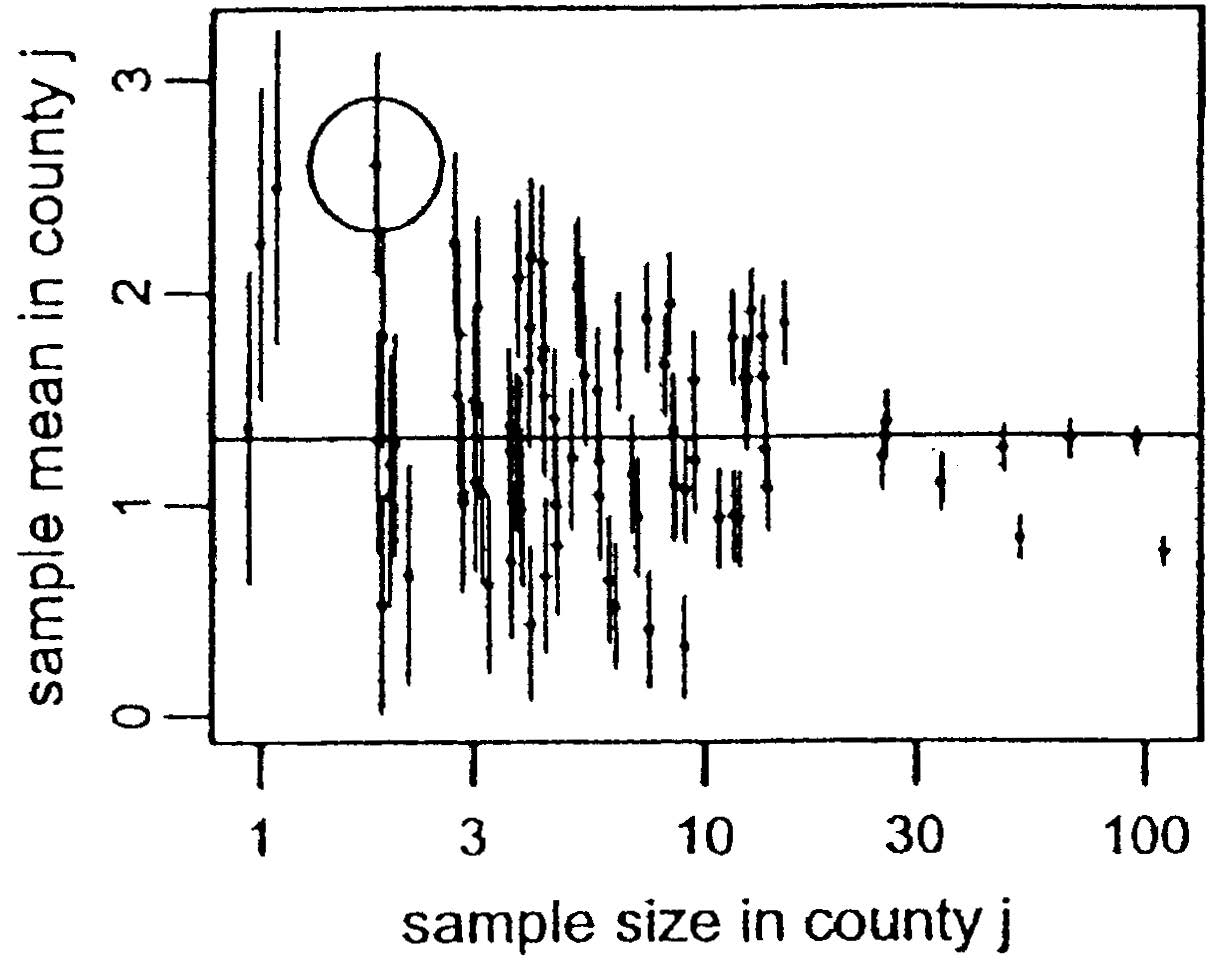
\includegraphics[width=0.50000\textwidth]{figures/gelmannopool.jpg}
\caption{Estimates and SE's for log radon levels in MN counties versus
the (jittered) sample size. The horizontal line indicates the overall
state mean (figure from Gelman and Hill).}
\end{figure}

Note we get pretty good (low variance) estimates in counties where more
samples were taken, while our estimates are not great in counties where
just a few samples were obtained.

\end{frame}

\begin{frame}{}

The figure contrasts two extreme approaches to obtaining estimates of
group means \(\mu_j\) in this type of setting. A common procedure might
be the following. Fit the ANOVA model
\(y_{ij}=\mu+\alpha_j+\varepsilon_{ij}\), where
\(\varepsilon_{ij} \sim N(0,\sigma^2)\), testing the significance of the
groups using an overall F test (here, an 84 degree of freedom test, as
we're testing all 85 means are the same).

\begin{itemize}
\tightlist
\item
  If \(p<0.05\), use the estimate \(\widehat{\mu}_j=\overline{y}_j\) for
  the mean in each county
\item
  If \(p>0.05\), use the estimate \(\widehat{\mu}_j=\overline{y}\) for
  the mean in each county
\end{itemize}

With either case, we will be using sub-optimal estimates for some
counties, and the above method is fairly extreme (all or nothing one way
or the other!).

\end{frame}

\begin{frame}{}

An improvement might be using the estimate \(\overline{y}_j\) for
counties with sufficient sample size and the estimate \(\overline{y}\)
for counties where the variability is too high.

Important question: how do we define ``sufficient'' and ``too high''?

\end{frame}

\begin{frame}{Random Effects ANOVA}

\emph{Random effects} ANOVA is a special case of a \emph{hierarchical}
or \emph{multilevel} linear model that provides a nice framework for
borrowing information across groups when needed to stabilize estimates.
We can specify such a model as \(y_{ij}=\mu+\alpha_j+\varepsilon_{ij}\),
where \(\varepsilon_{ij} \overset{iid}{\sim} N(0,\sigma^2)\) and
\(\alpha_j \overset{iid}{\sim} N(0,\tau^2)\). The model on \(\alpha_j\)
allows us to borrow information in order to obtain better group-specific
estimates when needed; because \(\alpha_j\) is now viewed as random, the
model can be called a \emph{random effects} model.

This particular model is sometimes called a \emph{random intercept}
model because each group has its own intercept, \(\mu_j=\mu+\alpha_j\),
that follows a Gaussian distribution.

\end{frame}

\begin{frame}{Random Effects ANOVA for Radon Data}

\begin{figure}
\centering
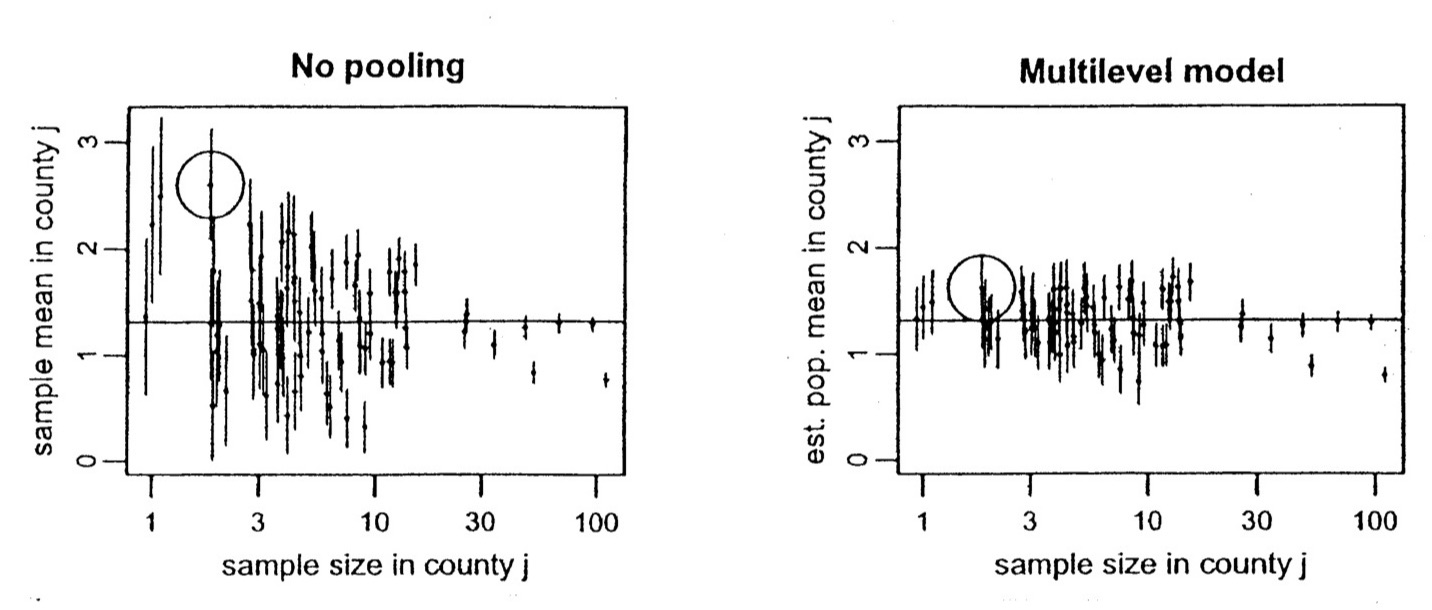
\includegraphics[width=0.50000\textwidth]{figures/gelman1.jpg}
\caption{Estimates and SE's for log radon levels in MN versus the
(jittered) sample size. The horizontal line indicates the complete
pooling estimate (Gelman and Hill). The circled data point had the
highest estimated mean radon level in fixed effects ANOVA.}
\end{figure}

\end{frame}

\begin{frame}{Radon study}

The multilevel estimates in the previous slide represent a compromise
between the two extremes. In this simple setting (with no predictors),
the multilevel estimate for county \(j\) can be approximated as a
weighted average of the mean of all observations in the county,
weighting both the unpooled estimate \(\overline{y}_j\) and the mean
over all counties \(\overline{y}\).

\end{frame}

\begin{frame}{}

How does random effects ANOVA borrow information?

The multilevel estimate

\[\widehat{\alpha}_j \approx
\frac{\frac{n_j}{\sigma^2}\overline{y}_j+\frac{1}{\tau^2}\overline{y}}{\frac{n_j}{\sigma^2}+\frac{1}{\tau^2}},\]

where

\begin{itemize}
\item
  \(n_j\) is the number of homes measured in county \(j\)
\item
  \(\sigma^2\) is the within-county variance in the log radon
  measurements
\item
  \(\tau^2\) is the variance across the average log radon levels of
  different counties
\end{itemize}

\end{frame}

\begin{frame}{}

The weighted average reflects the relative amount of information
available on each individual county, compared to that available across
all counties.

\begin{itemize}
\item
  Averages from counties with smaller sample sizes are less precise, so
  the weighting shrinks the multilevel estimates closer to the overall
  state average. For example, if \(n_j=0,\) the multilevel estimate is
  just \(\overline{y}\).
\item
  Averages from counties with larger sample sizes are more precise, and
  the multilevel estimates are closer to the county averages. As
  \(n_j \rightarrow \infty\), the multilevel estimate is just the county
  average \(\overline{y}_j\).
\item
  In intermediate cases, the multilevel estimate is in between the
  extremes.
\end{itemize}

In practice, we carry out all estimation together (estimate variances
along with the mean parameters), but we won't worry about this yet.

\end{frame}

\begin{frame}{Understanding the Model}

These estimates are often called \emph{shrinkage estimates}, as they
``shrink'' the no pooling estimates back towards the complete pooling
mean, to an extent determined by the information in the data.

Next we formalize the model and consider some of its features and
implications.

\end{frame}

\begin{frame}{Random Intercept Model}

This model is a special case of a \emph{random intercept} model in which
covariates are categorical. Note some consequences of this model.

\(y_{ij}=\mu+\alpha_j+\varepsilon_{ij}\), where
\(\varepsilon_{ij} \overset{iid}{\sim} N(0,\sigma^2)\) \(\perp\)
\(\alpha_j \overset{iid}{\sim} N(0,\tau^2)\)

\(E[y_{ij}]=E[\mu+\alpha_j+\varepsilon_{ij}]=\mu+0+0=\mu\)

\begin{eqnarray*}
\text{Var}[y_{ij}]&=&E[(y_{ij}-E(y_{ij}))^2] \\
&=& E[(\mu+\alpha_j+\varepsilon_{ij}-\mu)^2] \\
&=& E[(\alpha_j+\varepsilon_{ij})^2] \\
&=& E[\alpha_j^2+2\alpha_j\varepsilon_{ij}+\varepsilon_{ij}^2] \\
&=& \tau^2+0+\sigma^2=\sigma^2+\tau^2
\end{eqnarray*}

\end{frame}

\begin{frame}{}

For two observations in different groups j and j',

\begin{eqnarray*}
\text{Cov}(y_{ij},y_{i'j'})&=& E[(y_{ij}-E(y_{ij}))(y_{i'j'}-E(y_{i'j'}))] \\
&=& E(y_{ij}y_{i'j'})-\mu^2-\mu^2+\mu^2 \\
&=& E(y_{ij})E(y_{i'j'})-\mu^2=\mu^2-\mu^2=0
\end{eqnarray*}

\vspace{.1in}

For two observations in the same group j,

\begin{eqnarray*}
\text{Cov}(y_{ij},y_{i'j})&=& E[(y_{ij}-E(y_{ij}))(y_{i'j}-E(y_{i'j}))] \\
&=& E(y_{ij}y_{i'j})-\mu^2-\mu^2+\mu^2 \\
&=& E[(\mu+\alpha_j+\varepsilon_{ij})(\mu+\alpha_j + \varepsilon_{i'j})] \\
&=& E[\mu^2+\mu\alpha_j+\mu\varepsilon_{i'j}+\alpha_j\mu+\alpha_j^2+\alpha_j\varepsilon_{i'j}+ \\
& & ~~~~~\varepsilon_{ij}\mu+\varepsilon_{ij}\alpha_j+\varepsilon_{ij}\varepsilon_{i'j}] \\ 
&=& \mu^2 + 0 + 0 + 0 + \tau^2 + 0 + 0 + 0 + 0 -\mu^2=\tau^2
\end{eqnarray*}

\end{frame}

\begin{frame}{Intraclass Correlation}

The correlation between two observations in the same group is then given
by

\begin{eqnarray*}
\text{Corr}(y_{ij},y_{i'j})&=&\frac{\text{Cov}(y_{ij},y_{i'j})}{\sqrt(\text{Var}(y_{ij}))\sqrt(\text{Var}(y_{i'j}))} \\
&=& \frac{\tau^2}{\sigma^2+\tau^2}
\end{eqnarray*}

This motivates the use of random effects ANOVA to handle cases in which
we expect subgroups of observations to be correlated (e.g., repeated
measures or family studies).

\end{frame}

\begin{frame}{}

It is often convenient to stack our observations into a long vector
\(Y_{N \times 1}\) organized by groups. For simplicity in exposition,
assume \(n_j=n\) and the total sample size \(N=nJ\). Then assuming \(Y\)
follows a multivariate normal distribution (which follows from our
specification previously), we can express
\[\text{Cov}(Y)=\sigma^2I_{N\times N} + \tau^2 \begin{pmatrix} J_n & 0 & \cdots & 0 \\ 0 & J_n & \cdots & 0 \\
\vdots & \vdots & \vdots & \vdots \\ 0 & 0 & \cdots & J_n \end{pmatrix}=I_J \otimes V,\]
where \(V=\sigma^2I_n+\tau^2J_n\) and \(J_n\) is an \(n \times n\)
matrix of 1's.

\end{frame}

\begin{frame}{Kronecker product}

The \emph{Kronecker product} is a convenient way to express patterned
covariance matrices (among other things). For matrices
\(A_{m \times n}\) and \(B_{p \times q}\), the \emph{Kronecker product}
\(A \otimes B=\begin{bmatrix}a_{11}B & \cdots & a_{1n}B \\ \vdots & \ddots & \vdots \\ a_{m1}B & \cdots & a_{mn}B \end{bmatrix}\).

Using a Kronecker product, we can succinctly express the block diagonal
covariance matrix of all our observations when we have equal numbers of
observations in each group.

\end{frame}

\begin{frame}{Estimation Methods}

We briefly consider the following estimation methods for random
intercept models.

\begin{itemize}
\item
  Maximum likelihood (ML)
\item
  Restricted maximum likelihood (REML)
\item
  Empirical Bayes estimation
\end{itemize}

\end{frame}

\begin{frame}{Maximum Likelihood Estimation}

We can also think of this formulation in the framework of the general
linear mixed effects model, where \[y=X\beta+Zb+\varepsilon.\] In the
random effects ANOVA case,

\begin{itemize}
\tightlist
\item
  \(X\) is just a column of 1's specifying the intercept \(\beta=\mu\)
\item
  \(Z\) is a matrix of indicator variables indicating group membership
\item
  Assume the random effects \(b \sim N(0,G)\) where \(G=\tau^2I\) and
  the errors \(\varepsilon \sim N(0,R)\) where \(R=\sigma^2I\)
\end{itemize}

The covariance matrix \(\Sigma\) is then given by

\begin{eqnarray*}
\Sigma&=&\text{Var}(y)=\text{Var}(X\beta+Zb+\varepsilon) \\
&=& \text{Var}(X\beta)+\text{Var}(Zb)+\text{Var}(\varepsilon)  \\
&=& Z\text{Var}(b)Z' + \text{Var}(\varepsilon) = ZGZ'+R =\tau^2ZZ'+\sigma^2I
\end{eqnarray*}

\end{frame}

\begin{frame}{}

Assuming our \(N\) outcomes follow the multivariate Gaussian
distribution, our likelihood is given by
\[\frac{1}{(2\pi)^\frac{N}{2}|\Sigma|^\frac{1}{2}}\exp\left(-\frac{1}{2}(y-X\beta)'\Sigma^{-1}(y-X\beta)\right),\]

and we often work with the log-likelihood, given by

\begin{eqnarray*}
\ell(y,\beta,\Sigma)&=&-\frac{1}{2}\left\{N\log(2\pi) + \log |\Sigma| + (y-X\beta)'\Sigma^{-1}(y-X\beta)   \right\} \\
&\propto& \log |\Sigma| + (y-X\beta)'\Sigma^{-1}(y-X\beta),
\end{eqnarray*}

which we then minimize (as I took the negative) in order to find the
MLE.

\end{frame}

\begin{frame}{MLE for Bike Data}

Recall our model

\(y_{ij}=\mu+\alpha_j+\varepsilon_{ij}\), where
\(\varepsilon_{ij} \overset{iid}{\sim} N(0,\sigma^2)\) \(\perp\)
\(\alpha_j \overset{iid}{\sim} N(0,\tau^2)\), where \(y_{ij}\) indicates
the passing distance between the car and the bike, and \(\alpha_j\)
represent effects of different distances between the bike and the curb.

\end{frame}

\begin{frame}[fragile]{}

Instead of directly maximizing the log-likelihood in R, we can use the
lme4 library to do the work for us.

\begin{Shaded}
\begin{Highlighting}[]
\KeywordTok{load}\NormalTok{(}\StringTok{"~/Documents/GitHub/STA-410-610/PsychBikeData.RData"}\NormalTok{)}
\KeywordTok{library}\NormalTok{(lme4)}
\NormalTok{fit.ml=}\KeywordTok{lmer}\NormalTok{(}\StringTok{`}\DataTypeTok{passing distance}\StringTok{`} \OperatorTok{~}\StringTok{ }\NormalTok{(}\DecValTok{1} \OperatorTok{|}\StringTok{ }\NormalTok{kerb), }\DataTypeTok{REML=}\OtherTok{FALSE}\NormalTok{, }\DataTypeTok{data =}\NormalTok{ PsychBikeData)}
\KeywordTok{summary}\NormalTok{(fit.ml)}
\end{Highlighting}
\end{Shaded}

\end{frame}

\begin{frame}[fragile]{}

\begin{verbatim}
## Warning: package 'lme4' was built under R version 3.5.2
\end{verbatim}

\begin{verbatim}
## Loading required package: Matrix
\end{verbatim}

\begin{verbatim}
## Warning: package 'Matrix' was built under R version 3.5.2
\end{verbatim}

\begin{verbatim}
## Linear mixed model fit by maximum likelihood  ['lmerMod']
## Formula: `passing distance` ~ (1 | kerb)
##    Data: PsychBikeData
## 
##      AIC      BIC   logLik deviance df.resid 
##   2028.7   2046.0  -1011.4   2022.7     2352 
## 
## Scaled residuals: 
##     Min      1Q  Median      3Q     Max 
## -3.5113 -0.6674 -0.0948  0.5511  6.3949 
## 
## Random effects:
##  Groups   Name        Variance Std.Dev.
##  kerb     (Intercept) 0.009206 0.09595 
##  Residual             0.137203 0.37041 
## Number of obs: 2355, groups:  kerb, 5
## 
## Fixed effects:
##             Estimate Std. Error t value
## (Intercept)  1.54023    0.04363    35.3
\end{verbatim}

Our ML estimates of \((\mu,\tau^2,\sigma^2)\) for the bike data are
\((\widehat{\mu},\widehat{\tau}^2,\widehat{\sigma}^2)=(1.540, 0.009, 0.137)\)

\end{frame}

\begin{frame}{Fixed Effects ANOVA Table}

Previously, we examined an ANOVA table in which group \(j\) had \(n_j\)
members. For simplicity now assume \(n_j=n ~\forall ~ j\) so that N=Jn.
Then our ANOVA table can be written

\begin{longtable}[]{@{}llllll@{}}
\toprule
Source & DF & SS & MS & F & p\tabularnewline
\midrule
\endhead
Groups & \(J-1\) & SSG & \(MSG=\frac{SSG}{J-1}\) & \(\frac{MSG}{MSE}\) &
from \(F_{J-1,J(n-1)}\)\tabularnewline
Error & \(J(n-1)\) & SSE & \(MSE=\frac{SSE}{J(n-1)}\) & &\tabularnewline
Total & \(Jn-1\) & SST & & &\tabularnewline
\bottomrule
\end{longtable}

Our justification for the F ratio measuring evidence against \(H_0\) was
that

\begin{itemize}
\tightlist
\item
  \$E{[}MSE \mid \mu, \alpha\_j,\sigma\^{}2{]}=\sigma\^{}2
\item
  \(E[MSG \mid \mu, \alpha_j, \sigma^2]=\sigma^2+\frac{n\sum (\mu_j-\mu)^2}{J-1}\)
  (assuming equal group sizes)
\end{itemize}

\end{frame}

\begin{frame}{}

If we now treat \(\alpha_j \overset{iid}{\sim} N(0,\tau^2)\) as random,
then

\begin{eqnarray*}
E[MSG \mid \mu, \sigma^2, \tau^2]&=&E\left[E[MSG \mid \mu, \alpha_j, \sigma^2]\mid \mu, \sigma^2, \tau^2 \right] \\
&=& E[\sigma^2+\frac{n\sum (\mu_j-\mu)^2}{J-1}\mid \mu, \sigma^2, \tau^2]$ \\
&=& \sigma^2+n\tau^2
\end{eqnarray*}

because \(\frac{\sum (\mu_j-\mu)^2}{J-1}\) is an unbiased estimate of
\(\tau^2\). Thus
\(E[\frac{MSG-MSE}{n}]=(\sigma^2+n\tau^2-\sigma^2)/n=\tau^2\) and thus
an \emph{unbiased} estimate of \(\tau^2\) is given by
\(\widehat{\tau}^2=(MSG-MSE)/n\). This estimator has many names,
including

\begin{itemize}
\tightlist
\item
  ANOVA estimator (comes from ANOVA table)
\item
  method of moments estimator (based on expectations/moments)
\item
  restricted maximum likelihood (REML) estimator
\end{itemize}

\end{frame}

\begin{frame}{REML}

REML estimation is quite popular for variance component estimation.
Features of REML estimation include the following

\begin{itemize}
\tightlist
\item
  it is based on a likelihood function of residuals and therefore only
  uses information that does not depend on fixed effects
\item
  when all groups have the same sample size \(n_j=n\), it is the same as
  the ANOVA estimator
\end{itemize}

We'll get into more detail on REML estimation methods later in the
course -- it turns out our old friend \(s^2\) for the variance of a
normal distribution is a REML estimator.

\end{frame}

\begin{frame}[fragile]{REML Estimates for the Bike Data}

\begin{Shaded}
\begin{Highlighting}[]
\NormalTok{fit.reml=}\KeywordTok{lmer}\NormalTok{(}\StringTok{`}\DataTypeTok{passing distance}\StringTok{`} \OperatorTok{~}\StringTok{ }\NormalTok{(}\DecValTok{1} \OperatorTok{|}\StringTok{ }\NormalTok{kerb), }\DataTypeTok{REML=}\OtherTok{TRUE}\NormalTok{, }\DataTypeTok{data =}\NormalTok{ PsychBikeData)}
\KeywordTok{summary}\NormalTok{(fit.reml)}
\end{Highlighting}
\end{Shaded}

\begin{verbatim}
## Linear mixed model fit by REML ['lmerMod']
## Formula: `passing distance` ~ (1 | kerb)
##    Data: PsychBikeData
## 
## REML criterion at convergence: 2027
## 
## Scaled residuals: 
##     Min      1Q  Median      3Q     Max 
## -3.5132 -0.6647 -0.0940  0.5498  6.3978 
## 
## Random effects:
##  Groups   Name        Variance Std.Dev.
##  kerb     (Intercept) 0.01157  0.1076  
##  Residual             0.13720  0.3704  
## Number of obs: 2355, groups:  kerb, 5
## 
## Fixed effects:
##             Estimate Std. Error t value
## (Intercept)  1.54008    0.04876   31.59
\end{verbatim}

Our REML estimates for the bike data are
\((\widehat{\mu},\widehat{\tau}^2,\widehat{\sigma}^2)=(1.540, 0.012, 0.137)\).

\end{frame}

\begin{frame}{}

Note that the ``REML'' estimate of the mean \(\mu\) is not obtained
using the REML likelihood, which does not involve parameters in the
linear predictor. We will return to this point later in the course.

\end{frame}

\begin{frame}{Empirical Bayes}

Recall our group means formulation:

\begin{eqnarray*}
y_{ij}&=&\mu_j+\varepsilon_{ij}\\
\mu_1,\cdots,\mu_J &\overset{iid}{\sim}& N(\mu, \tau^2) \\
\varepsilon_{ij} &\overset{iid}{\sim} & N(0,\sigma^2).
\end{eqnarray*}

Suppose \((\mu, \tau^2, \sigma^2)\) are known exactly and consider
estimating \(\mu_j\) with an estimator that is a linear function of the
group sample mean \(\widehat{\mu}_j=a\overline{y}_j+b\). Then one can
show that the MSE \(E[(\mu_j-\widehat{\mu}_j)^2]\) is minimized if
\(a=\frac{\frac{n_j}{\sigma^2}}{\frac{n_j}{\sigma^2}+\frac{1}{\tau^2}}\)
and \(b=(1-a)\mu\), so that
\(\widehat{\mu}_j=w_j \overline{y}_j+(1-w_j)\mu\), where
\(w_j=\frac{\frac{n_j}{\sigma^2}}{\frac{n_j}{\sigma^2}+\frac{1}{\tau^2}}\)

\end{frame}

\begin{frame}{}

If we knew \((\mu, \tau^2,\sigma^2)\) this estimate would be the
\emph{Bayes estimate}; however, we do not know these parameters and are
instead estimating them from the data, so that

\(\widehat{\mu}_j=\widehat{w}_j \overline{y}_j+(1-\widehat{w}_j)\widehat{\mu}\),
where
\(\widehat{w}_j=\frac{\frac{n_j}{\widehat{\sigma}^2}}{\frac{n_j}{\widehat{\sigma}^2}+\frac{1}{\widehat{\tau}^2}}\)

is called an \emph{empirical Bayes estimate} because our unknown
parameters have been replaced by ``empirical'' estimates from the data.

\end{frame}

\begin{frame}[fragile]{EB Estimates of Group Means for Bike Data}

\begin{Shaded}
\begin{Highlighting}[]
\KeywordTok{tapply}\NormalTok{(PsychBikeData}\OperatorTok{$}\StringTok{`}\DataTypeTok{passing distance}\StringTok{`}\NormalTok{,PsychBikeData}\OperatorTok{$}\NormalTok{kerb,mean)}
\end{Highlighting}
\end{Shaded}

\begin{verbatim}
##     0.25      0.5     0.75        1     1.25 
## 1.698054 1.590473 1.505519 1.490584 1.412813
\end{verbatim}

\begin{Shaded}
\begin{Highlighting}[]
\KeywordTok{coef}\NormalTok{(fit.ml)}
\end{Highlighting}
\end{Shaded}

\begin{verbatim}
## $kerb
##      (Intercept)
## 0.25    1.694619
## 0.5     1.589136
## 0.75    1.506981
## 1       1.492113
## 1.25    1.418287
## 
## attr(,"class")
## [1] "coef.mer"
\end{verbatim}

\end{frame}

\begin{frame}[fragile]{}

\begin{Shaded}
\begin{Highlighting}[]
\KeywordTok{tapply}\NormalTok{(PsychBikeData}\OperatorTok{$}\StringTok{`}\DataTypeTok{passing distance}\StringTok{`}\NormalTok{,PsychBikeData}\OperatorTok{$}\NormalTok{kerb,mean)}
\end{Highlighting}
\end{Shaded}

\begin{verbatim}
##     0.25      0.5     0.75        1     1.25 
## 1.698054 1.590473 1.505519 1.490584 1.412813
\end{verbatim}

\begin{Shaded}
\begin{Highlighting}[]
\KeywordTok{coef}\NormalTok{(fit.reml)}
\end{Highlighting}
\end{Shaded}

\begin{verbatim}
## $kerb
##      (Intercept)
## 0.25    1.695307
## 0.5     1.589401
## 0.75    1.506687
## 1       1.491805
## 1.25    1.417201
## 
## attr(,"class")
## [1] "coef.mer"
\end{verbatim}

\end{frame}

\begin{frame}{Data exploration in Radon Study}

\begin{figure}
\centering
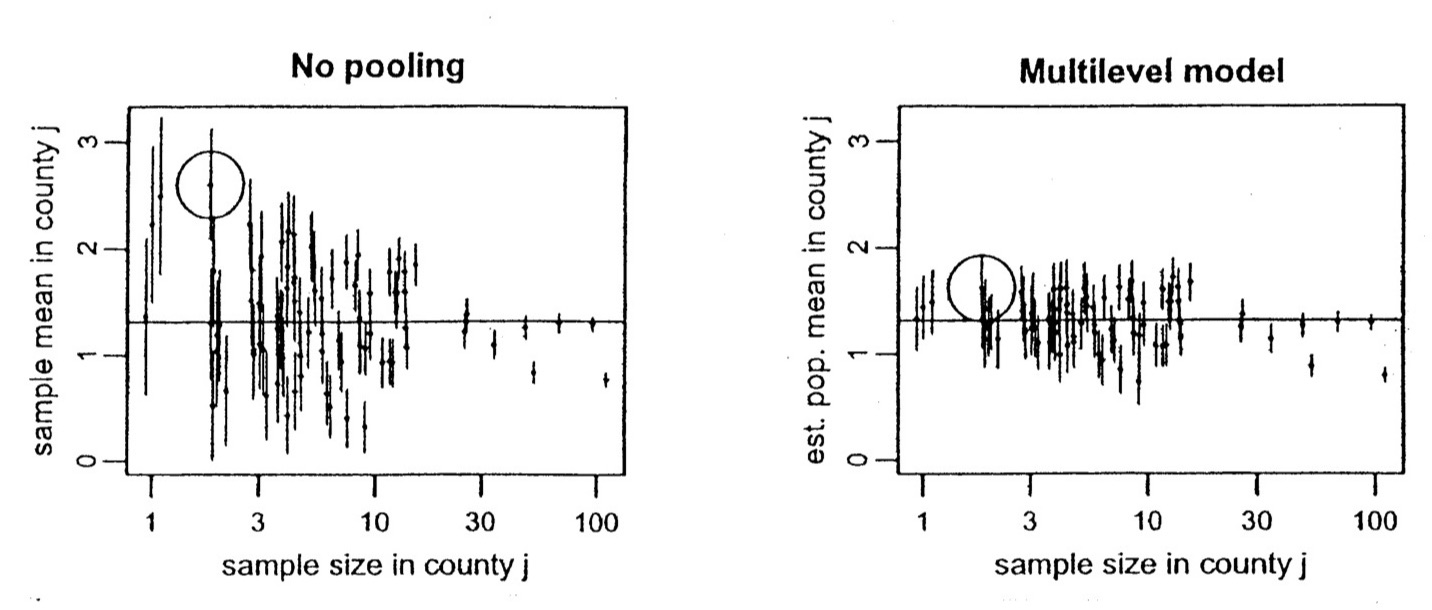
\includegraphics[width=0.70000\textwidth]{figures/gelman1.jpg}
\caption{Estimates and SE's for log radon levels in MN versus the
(jittered) sample size. The horizontal line indicates the complete
pooling estimate (Gelman and Hill).}
\end{figure}

\end{frame}

\begin{frame}{Radon study}

The multilevel estimates in the previous slide represent a compromise
between the two extremes. In this simple setting (with no predictors),
the multilevel estimate for county \(j\) can be approximated as a
weighted average of the mean of all observations in the county,
weighting both the unpooled estimate \(\overline{y}_j\) and the mean
over all counties \(\overline{y}_{\cdot \cdot}\).

\end{frame}

\begin{frame}{Radon study}

\[\widehat{\alpha}_j \approx
\frac{\frac{n_j}{\sigma^2_y}\overline{y}_j+\frac{1}{\sigma^2_{\alpha}}\overline{y}_{\cdot\cdot}}{\frac{n_j}{\sigma^2_y}+\frac{1}{\sigma^2_{\alpha}}},\]
where

\begin{itemize}
\item
  \(n_j\) is the number of homes measured in county \(j\)
\item
  \(\sigma^2_y\) is the within-county variance in the log radon
  measurements
\item
  \(\sigma^2_{\alpha}\) is the variance across the average log radon
  levels of different counties
\end{itemize}

\end{frame}

\begin{frame}{Radon study}

The weighted average reflects the relative amount of information
available on each individual county, compared to that available across
all counties.

\begin{itemize}
\item
  Averages from counties with smaller sample sizes are less precise, so
  the weighting shrinks the multilevel estimates closer to the overall
  state average. For example, if \(n_j=0,\) the multilevel estimate is
  just \(\overline{y}_{\cdot \cdot}\).
\item
  Averages from counties with larger sample sizes are more precise, and
  the multilevel estimates are closer to the county averages. As
  \(n_j \rightarrow \infty\), the multilevel estimate is just the county
  average \(\overline{y}_j\).
\item
  In intermediate cases, the multilevel estimate is in between the
  extremes.
\end{itemize}

\end{frame}

\begin{frame}{Radon study}

In practice, we carry out all estimation together (estimate variances
along with the \(\alpha\) parameters), but we won't worry about this
yet.

Code for the radon analysis as presented in Gelman and Hill
\href{http://www.stat.columbia.edu/~gelman/arm/examples/radon/radon_chap12.R}{is
available at this link} .

\end{frame}

\begin{frame}{Adding a Grouping Factor: Location of Measurement}

One important predictor of radon levels is the floor on which the
measurement is taken: basement (\(x_i=0\)) or first floor (\(x_i=1\)).
Radon comes from underground and can enter more easily when the house is
built into the ground; in addition, basements tend to have higher levels
than ground floors.

First, we examine the complete-pooling regression,
\(y_i=\alpha+\beta x_i + \varepsilon_i\), and the no-pooling regression
\(y_i=\alpha_{j[i]}+\beta x_i + \varepsilon_i\), where \(\alpha_{j[i]}\)
is the mean log radon level from basement measures of homes (indexed by
i) in county \(j\).

The following plot shows the dashed lines
\(\widehat{y}=\widehat{\alpha}+\widehat{\beta} x\) for eight selected
counties from the complete pooling model, and the solid lines
\(\widehat{y}=\widehat{\alpha}_j+\widehat{\beta}x\) from no pooling
model.

\end{frame}

\begin{frame}{No pooling and pooling}

\begin{figure}
\centering
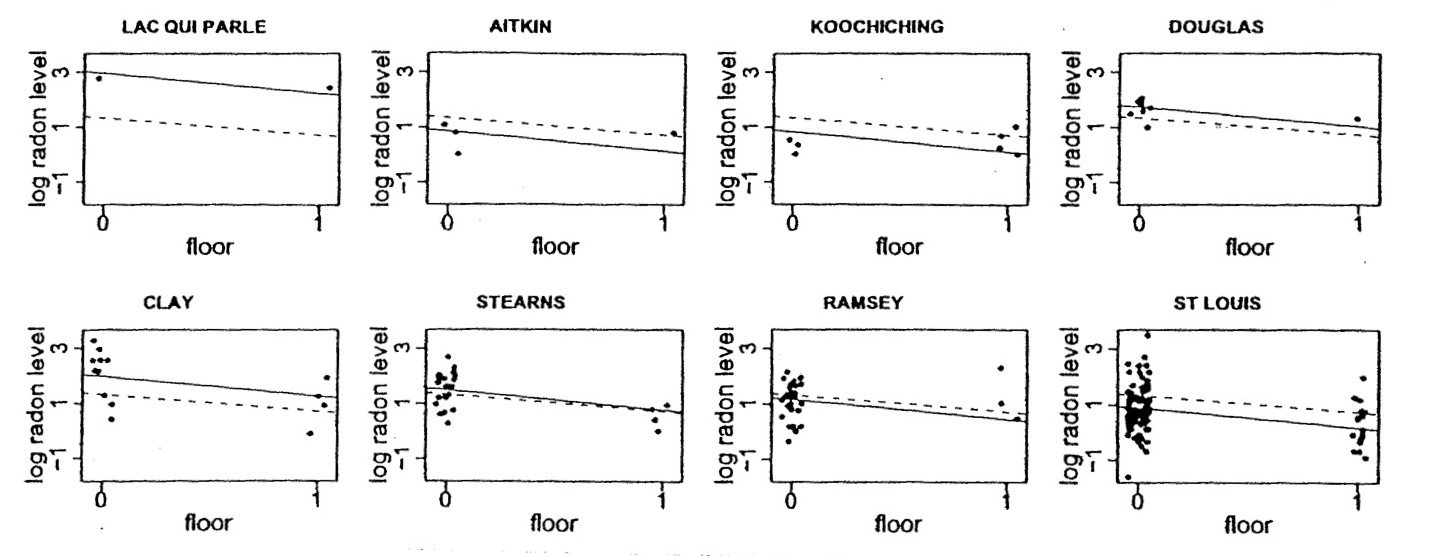
\includegraphics[width=0.70000\textwidth]{figures/gelman2.jpg}
\caption{Complete-pooling (dashed) and no-pooling (solid) regression
fits to radon data (Gelman and Hill)}
\end{figure}

\end{frame}

\begin{frame}{Interpretation}

The estimates of \(\beta\) (the association between floor of home and
radon level) differ slightly for the two regressions, with
\(\widehat{\beta}=-0.61\) for the pooling model, and
\(\widehat{\beta}=-0.72\) for the no-pooling model. As we might expect,
we tend to have higher radon levels in the basement
(p\textless{}0.0001). (Note: the models differ a LOT in adjusted
\(R^2\): 0.07 in the complete pooling model, and 0.74 in the no pooling
model.)

Neither analysis is perfect. The complete-pooling analysis ignores
variation in radon levels between counties, which is undesirable because
our goal is to identify counties with high-radon homes -- we can't pool
away the main research question! The no-pooling analysis is also
problematic -- for example the Lac Qui Parle County line is estimated
based on just two data points.

\end{frame}

\begin{frame}{Multilevel model}

We will start with a simple multilevel model,
\(y_i=\gamma_0 + \alpha_{j[i]}+\beta x_i + \varepsilon_i\), where now
\(\alpha_{j} \sim N(0,\sigma^2_\alpha)\) and
\(\varepsilon_i \sim N(0, \sigma^2_y)\). We fit this model using the
lmer() function in the lme4 package.

This model can also be written
\(y_i \sim N(\alpha_{j[i]}+\beta x_i, \sigma_y^2),\)

\(\alpha_j \sim N\left(\gamma_0,\sigma_\alpha^2 \right)\)

\end{frame}

\begin{frame}[fragile]{Code to fit models}

\begin{Shaded}
\begin{Highlighting}[]
\NormalTok{srrs2 <-}\StringTok{ }\KeywordTok{read.table}\NormalTok{ (}\StringTok{"data/srrs2.dat"}\NormalTok{, }\DataTypeTok{header=}\NormalTok{T, }\DataTypeTok{sep=}\StringTok{","}\NormalTok{)}
\NormalTok{mn <-}\StringTok{ }\NormalTok{srrs2}\OperatorTok{$}\NormalTok{state}\OperatorTok{==}\StringTok{"MN"}
\NormalTok{radon <-}\StringTok{ }\NormalTok{srrs2}\OperatorTok{$}\NormalTok{activity[mn]}
\NormalTok{log.radon <-}\StringTok{ }\KeywordTok{log}\NormalTok{ (}\KeywordTok{ifelse}\NormalTok{ (radon}\OperatorTok{==}\DecValTok{0}\NormalTok{, .}\DecValTok{1}\NormalTok{, radon))}
\NormalTok{floor <-}\StringTok{ }\NormalTok{srrs2}\OperatorTok{$}\NormalTok{floor[mn]   }\CommentTok{# 0 for basement, 1 for first floor}
\NormalTok{n <-}\StringTok{ }\KeywordTok{length}\NormalTok{(radon)}
\NormalTok{y <-}\StringTok{ }\NormalTok{log.radon}
\NormalTok{x <-}\StringTok{ }\NormalTok{floor}

\NormalTok{county.name <-}\StringTok{ }\KeywordTok{as.vector}\NormalTok{(srrs2}\OperatorTok{$}\NormalTok{county[mn])}
\NormalTok{uniq <-}\StringTok{ }\KeywordTok{unique}\NormalTok{(county.name)}
\NormalTok{J <-}\StringTok{ }\KeywordTok{length}\NormalTok{(uniq)}
\NormalTok{county <-}\StringTok{ }\KeywordTok{rep}\NormalTok{ (}\OtherTok{NA}\NormalTok{, J)}
\ControlFlowTok{for}\NormalTok{ (i }\ControlFlowTok{in} \DecValTok{1}\OperatorTok{:}\NormalTok{J)\{}
\NormalTok{  county[county.name}\OperatorTok{==}\NormalTok{uniq[i]] <-}\StringTok{ }\NormalTok{i}
\NormalTok{\}}
\end{Highlighting}
\end{Shaded}

\begin{Shaded}
\begin{Highlighting}[]
\NormalTok{###pooled model}
\NormalTok{lm.pooled<-}\KeywordTok{lm}\NormalTok{(}\DataTypeTok{formula=}\NormalTok{y}\OperatorTok{~}\NormalTok{x)}
\KeywordTok{summary}\NormalTok{(lm.pooled)}
\NormalTok{###unpooled  model}
\NormalTok{lm.unpooled<-}\KeywordTok{lm}\NormalTok{(}\DataTypeTok{formula=}\NormalTok{y}\OperatorTok{~}\NormalTok{x}\OperatorTok{+}\KeywordTok{factor}\NormalTok{(county)}\OperatorTok{-}\DecValTok{1}\NormalTok{)}
\KeywordTok{summary}\NormalTok{(lm.unpooled)}
\end{Highlighting}
\end{Shaded}

\end{frame}

\begin{frame}[fragile]{}

\begin{verbatim}
## 
## Call:
## lm(formula = y ~ x)
## 
## Residuals:
##     Min      1Q  Median      3Q     Max 
## -3.6293 -0.5383  0.0342  0.5603  2.5486 
## 
## Coefficients:
##             Estimate Std. Error t value Pr(>|t|)    
## (Intercept)  1.32674    0.02972  44.640   <2e-16 ***
## x           -0.61339    0.07284  -8.421   <2e-16 ***
## ---
## Signif. codes:  0 '***' 0.001 '**' 0.01 '*' 0.05 '.' 0.1 ' ' 1
## 
## Residual standard error: 0.8226 on 917 degrees of freedom
## Multiple R-squared:  0.07178,    Adjusted R-squared:  0.07077 
## F-statistic: 70.91 on 1 and 917 DF,  p-value: < 2.2e-16
\end{verbatim}

\end{frame}

\begin{frame}[fragile]{}

\begin{verbatim}
## 
## Call:
## lm(formula = y ~ x + factor(county) - 1)
## 
## Residuals:
##      Min       1Q   Median       3Q      Max 
## -3.14595 -0.45405  0.00065  0.45376  2.65987 
## 
## Coefficients:
##                  Estimate Std. Error t value Pr(>|t|)    
## x                -0.72054    0.07352  -9.800  < 2e-16 ***
## factor(county)1   0.84054    0.37866   2.220 0.026701 *  
## factor(county)2   0.87482    0.10498   8.333 3.23e-16 ***
## factor(county)3   1.52870    0.43946   3.479 0.000530 ***
## factor(county)4   1.55272    0.28897   5.373 1.00e-07 ***
## factor(county)5   1.43257    0.37866   3.783 0.000166 ***
## factor(county)6   1.51301    0.43672   3.464 0.000558 ***
## factor(county)7   2.01216    0.20243   9.940  < 2e-16 ***
## factor(county)8   1.98958    0.37999   5.236 2.08e-07 ***
## factor(county)9   1.00304    0.23931   4.191 3.07e-05 ***
## factor(county)10  1.56391    0.31099   5.029 6.04e-07 ***
## factor(county)11  1.40113    0.33828   4.142 3.80e-05 ***
## factor(county)12  1.73025    0.37821   4.575 5.49e-06 ***
## factor(county)13  1.03872    0.30881   3.364 0.000804 ***
## factor(county)14  1.98838    0.20325   9.783  < 2e-16 ***
## factor(county)15  1.33797    0.37999   3.521 0.000453 ***
## factor(county)16  0.66486    0.53487   1.243 0.214204    
## factor(county)17  1.27480    0.38221   3.335 0.000890 ***
## factor(county)18  1.12155    0.21913   5.118 3.83e-07 ***
## factor(county)19  1.33831    0.09541  14.026  < 2e-16 ***
## factor(county)20  1.80032    0.43672   4.122 4.13e-05 ***
## factor(county)21  1.73399    0.25227   6.873 1.23e-11 ***
## factor(county)22  0.63679    0.30905   2.060 0.039663 *  
## factor(county)23  1.39999    0.53613   2.611 0.009183 ** 
## factor(county)24  2.10162    0.25267   8.318 3.64e-16 ***
## factor(county)25  1.95072    0.20243   9.636  < 2e-16 ***
## factor(county)26  1.36058    0.07422  18.332  < 2e-16 ***
## factor(county)27  1.77336    0.30978   5.725 1.45e-08 ***
## factor(county)28  1.24159    0.34115   3.639 0.000290 ***
## factor(county)29  1.05600    0.43672   2.418 0.015818 *  
## factor(county)30  0.92576    0.22807   4.059 5.39e-05 ***
## factor(county)31  2.02057    0.33828   5.973 3.45e-09 ***
## factor(county)32  1.23629    0.37821   3.269 0.001124 ** 
## factor(county)33  2.06187    0.37821   5.452 6.58e-08 ***
## factor(county)34  1.59044    0.43946   3.619 0.000314 ***
## factor(county)35  0.81920    0.28897   2.835 0.004695 ** 
## factor(county)36  2.95897    0.53613   5.519 4.55e-08 ***
## factor(county)37  0.40209    0.25227   1.594 0.111345    
## factor(county)38  1.86772    0.37999   4.915 1.07e-06 ***
## factor(county)39  1.74807    0.33860   5.163 3.05e-07 ***
## factor(county)40  2.31580    0.37866   6.116 1.48e-09 ***
## factor(county)41  1.96715    0.26759   7.351 4.69e-13 ***
## factor(county)42  1.36098    0.75642   1.799 0.072343 .  
## factor(county)43  1.60224    0.25543   6.273 5.69e-10 ***
## factor(county)44  1.04099    0.28609   3.639 0.000291 ***
## factor(county)45  1.29541    0.21101   6.139 1.28e-09 ***
## factor(county)46  1.21461    0.33828   3.591 0.000349 ***
## factor(county)47  0.88393    0.53613   1.649 0.099583 .  
## factor(county)48  1.14812    0.25227   4.551 6.13e-06 ***
## factor(county)49  1.70211    0.21010   8.102 1.93e-15 ***
## factor(county)50  2.49321    0.75642   3.296 0.001022 ** 
## factor(county)51  2.16504    0.37821   5.724 1.45e-08 ***
## factor(county)52  1.92769    0.43672   4.414 1.15e-05 ***
## factor(county)53  1.25080    0.43741   2.860 0.004348 ** 
## factor(county)54  1.30676    0.15802   8.270 5.28e-16 ***
## factor(county)55  1.61799    0.26885   6.018 2.64e-09 ***
## factor(county)56  1.10110    0.43946   2.506 0.012415 *  
## factor(county)57  0.76218    0.30905   2.466 0.013855 *  
## factor(county)58  1.86092    0.37866   4.915 1.07e-06 ***
## factor(county)59  1.72178    0.37999   4.531 6.73e-06 ***
## factor(county)60  1.27939    0.53487   2.392 0.016979 *  
## factor(county)61  1.15873    0.13389   8.654  < 2e-16 ***
## factor(county)62  1.98301    0.33860   5.856 6.80e-09 ***
## factor(county)63  1.67070    0.43741   3.820 0.000144 ***
## factor(county)64  1.84784    0.22817   8.099 1.97e-15 ***
## factor(county)65  1.29912    0.53487   2.429 0.015357 *  
## factor(county)66  1.66574    0.20648   8.067 2.50e-15 ***
## factor(county)67  1.80312    0.21101   8.545  < 2e-16 ***
## factor(county)68  1.09002    0.26743   4.076 5.02e-05 ***
## factor(county)69  1.24245    0.37821   3.285 0.001062 ** 
## factor(county)70  0.86763    0.07096  12.227  < 2e-16 ***
## factor(county)71  1.49184    0.15174   9.832  < 2e-16 ***
## factor(county)72  1.57990    0.23920   6.605 7.08e-11 ***
## factor(county)73  1.79176    0.53487   3.350 0.000845 ***
## factor(county)74  0.98704    0.37821   2.610 0.009223 ** 
## factor(county)75  1.72372    0.43741   3.941 8.80e-05 ***
## factor(county)76  2.00844    0.37866   5.304 1.45e-07 ***
## factor(county)77  1.82168    0.28609   6.367 3.17e-10 ***
## factor(county)78  1.28569    0.33956   3.786 0.000164 ***
## factor(county)79  0.61488    0.37866   1.624 0.104785    
## factor(county)80  1.32952    0.11181  11.890  < 2e-16 ***
## factor(county)81  2.70953    0.43946   6.166 1.09e-09 ***
## factor(county)82  2.23001    0.75642   2.948 0.003286 ** 
## factor(county)83  1.62292    0.21048   7.711 3.57e-14 ***
## factor(county)84  1.64535    0.20987   7.840 1.38e-14 ***
## factor(county)85  1.18652    0.53487   2.218 0.026801 *  
## ---
## Signif. codes:  0 '***' 0.001 '**' 0.01 '*' 0.05 '.' 0.1 ' ' 1
## 
## Residual standard error: 0.7564 on 833 degrees of freedom
## Multiple R-squared:  0.7671, Adjusted R-squared:  0.7431 
## F-statistic: 31.91 on 86 and 833 DF,  p-value: < 2.2e-16
\end{verbatim}

\end{frame}

\begin{frame}[fragile]{}

\begin{Shaded}
\begin{Highlighting}[]
\CommentTok{#basic MLM with just random intercept for county}
\KeywordTok{library}\NormalTok{(lme4)}
\NormalTok{M1<-}\KeywordTok{lmer}\NormalTok{(y}\OperatorTok{~}\NormalTok{x}\OperatorTok{+}\NormalTok{(}\DecValTok{1}\OperatorTok{|}\NormalTok{county),}\DataTypeTok{REML=}\OtherTok{FALSE}\NormalTok{)}
\KeywordTok{summary}\NormalTok{(M1)}
\KeywordTok{coef}\NormalTok{(M1)}
\end{Highlighting}
\end{Shaded}

\end{frame}

\begin{frame}[fragile]{}

\begin{verbatim}
## Linear mixed model fit by maximum likelihood  ['lmerMod']
## Formula: y ~ x + (1 | county)
## 
##      AIC      BIC   logLik deviance df.resid 
##   2171.7   2190.9  -1081.8   2163.7      915 
## 
## Scaled residuals: 
##     Min      1Q  Median      3Q     Max 
## -4.4071 -0.6164  0.0056  0.6398  3.4288 
## 
## Random effects:
##  Groups   Name        Variance Std.Dev.
##  county   (Intercept) 0.1053   0.3245  
##  Residual             0.5703   0.7552  
## Number of obs: 919, groups:  county, 85
## 
## Fixed effects:
##             Estimate Std. Error t value
## (Intercept)  1.46116    0.05124  28.516
## x           -0.69264    0.07036  -9.844
## 
## Correlation of Fixed Effects:
##   (Intr)
## x -0.290
\end{verbatim}

\begin{verbatim}
## $county
##    (Intercept)          x
## 1    1.1945745 -0.6926365
## 2    0.9286777 -0.6926365
## 3    1.4786009 -0.6926365
## 4    1.5037889 -0.6926365
## 5    1.4460519 -0.6926365
## 6    1.4796397 -0.6926365
## 7    1.8555701 -0.6926365
## 8    1.6796893 -0.6926365
## 9    1.1621916 -0.6926365
## 10   1.5078244 -0.6926365
## 11   1.4323468 -0.6926365
## 12   1.5754595 -0.6926365
## 13   1.2391507 -0.6926365
## 14   1.8355525 -0.6926365
## 15   1.4029057 -0.6926365
## 16   1.2464311 -0.6926365
## 17   1.3731083 -0.6926365
## 18   1.2223643 -0.6926365
## 19   1.3464032 -0.6926365
## 20   1.5820437 -0.6926365
## 21   1.6295442 -0.6926365
## 22   1.0254760 -0.6926365
## 23   1.4409018 -0.6926365
## 24   1.8571106 -0.6926365
## 25   1.8112724 -0.6926365
## 26   1.3627354 -0.6926365
## 27   1.6203441 -0.6926365
## 28   1.3477310 -0.6926365
## 29   1.3167485 -0.6926365
## 30   1.1024167 -0.6926365
## 31   1.7296714 -0.6926365
## 32   1.3656408 -0.6926365
## 33   1.7163254 -0.6926365
## 34   1.5006074 -0.6926365
## 35   1.0902638 -0.6926365
## 36   1.8612907 -0.6926365
## 37   0.7980765 -0.6926365
## 38   1.6279261 -0.6926365
## 39   1.5961932 -0.6926365
## 40   1.8212249 -0.6926365
## 41   1.7607856 -0.6926365
## 42   1.4455459 -0.6926365
## 43   1.5395531 -0.6926365
## 44   1.2220391 -0.6926365
## 45   1.3381032 -0.6926365
## 46   1.3428173 -0.6926365
## 47   1.3017421 -0.6926365
## 48   1.2638020 -0.6926365
## 49   1.6282095 -0.6926365
## 50   1.6219929 -0.6926365
## 51   1.7601468 -0.6926365
## 52   1.6274442 -0.6926365
## 53   1.3828666 -0.6926365
## 54   1.3332417 -0.6926365
## 55   1.5484354 -0.6926365
## 56   1.3261923 -0.6926365
## 57   1.0913754 -0.6926365
## 58   1.6280045 -0.6926365
## 59   1.5659375 -0.6926365
## 60   1.4121426 -0.6926365
## 61   1.2002725 -0.6926365
## 62   1.7089656 -0.6926365
## 63   1.5325292 -0.6926365
## 64   1.7185497 -0.6926365
## 65   1.4174628 -0.6926365
## 66   1.5971714 -0.6926365
## 67   1.6964805 -0.6926365
## 68   1.2398624 -0.6926365
## 69   1.3682586 -0.6926365
## 70   0.8904344 -0.6926365
## 71   1.4827093 -0.6926365
## 72   1.5381798 -0.6926365
## 73   1.5503073 -0.6926365
## 74   1.2597664 -0.6926365
## 75   1.5514276 -0.6926365
## 76   1.6906647 -0.6926365
## 77   1.6621565 -0.6926365
## 78   1.3715768 -0.6926365
## 79   1.0987212 -0.6926365
## 80   1.3406745 -0.6926365
## 81   1.8994853 -0.6926365
## 82   1.5809771 -0.6926365
## 83   1.5707987 -0.6926365
## 84   1.5896624 -0.6926365
## 85   1.3871005 -0.6926365
## 
## attr(,"class")
## [1] "coef.mer"
\end{verbatim}

\begin{Shaded}
\begin{Highlighting}[]
\KeywordTok{library}\NormalTok{(lme4)}
\CommentTok{#basic MLM with just random intercept for county, fit using REML}
\NormalTok{M2<-}\KeywordTok{lmer}\NormalTok{(y}\OperatorTok{~}\NormalTok{x}\OperatorTok{+}\NormalTok{(}\DecValTok{1}\OperatorTok{|}\NormalTok{county))}
\end{Highlighting}
\end{Shaded}

\end{frame}

\begin{frame}[fragile]{Output from MLM}

\begin{Shaded}
\begin{Highlighting}[]
\KeywordTok{summary}\NormalTok{(M2)}
\end{Highlighting}
\end{Shaded}

\begin{verbatim}
## Linear mixed model fit by REML ['lmerMod']
## Formula: y ~ x + (1 | county)
## 
## REML criterion at convergence: 2171.3
## 
## Scaled residuals: 
##     Min      1Q  Median      3Q     Max 
## -4.3989 -0.6155  0.0029  0.6405  3.4281 
## 
## Random effects:
##  Groups   Name        Variance Std.Dev.
##  county   (Intercept) 0.1077   0.3282  
##  Residual             0.5709   0.7556  
## Number of obs: 919, groups:  county, 85
## 
## Fixed effects:
##             Estimate Std. Error t value
## (Intercept)  1.46160    0.05158  28.339
## x           -0.69299    0.07043  -9.839
## 
## Correlation of Fixed Effects:
##   (Intr)
## x -0.288
\end{verbatim}

 The ratio of county-level variance to total variance is an estimate of
the correlation of within-county measures. Here
\(\hat{\rho}=\frac{.1077}{.1077+.5709}=0.16\).

\end{frame}

\begin{frame}[fragile]{County-level estimates}

\begin{Shaded}
\begin{Highlighting}[]
\KeywordTok{coef}\NormalTok{(M2)}
\end{Highlighting}
\end{Shaded}

\begin{verbatim}
## $county
##    (Intercept)          x
## 1    1.1915004 -0.6929937
## 2    0.9276468 -0.6929937
## 3    1.4792143 -0.6929937
## 4    1.5045012 -0.6929937
## 5    1.4461503 -0.6929937
## 6    1.4801817 -0.6929937
## 7    1.8581255 -0.6929937
## 8    1.6827736 -0.6929937
## 9    1.1600747 -0.6929937
## 10   1.5086099 -0.6929937
## 11   1.4322449 -0.6929937
## 12   1.5771520 -0.6929937
## 13   1.2370518 -0.6929937
## 14   1.8380232 -0.6929937
## 15   1.4024982 -0.6929937
## 16   1.2432992 -0.6929937
## 17   1.3723633 -0.6929937
## 18   1.2209415 -0.6929937
## 19   1.3462611 -0.6929937
## 20   1.5840332 -0.6929937
## 21   1.6311136 -0.6929937
## 22   1.0211903 -0.6929937
## 23   1.4409443 -0.6929937
## 24   1.8605721 -0.6929937
## 25   1.8135585 -0.6929937
## 26   1.3626875 -0.6929937
## 27   1.6222663 -0.6929937
## 28   1.3467692 -0.6929937
## 29   1.3149879 -0.6929937
## 30   1.0999775 -0.6929937
## 31   1.7329562 -0.6929937
## 32   1.3646863 -0.6929937
## 33   1.7197950 -0.6929937
## 34   1.5015319 -0.6929937
## 35   1.0870316 -0.6929937
## 36   1.8680899 -0.6929937
## 37   0.7928242 -0.6929937
## 38   1.6303574 -0.6929937
## 39   1.5979922 -0.6929937
## 40   1.8260564 -0.6929937
## 41   1.7636308 -0.6929937
## 42   1.4456250 -0.6929937
## 43   1.5404841 -0.6929937
## 44   1.2199767 -0.6929937
## 45   1.3375197 -0.6929937
## 46   1.3416955 -0.6929937
## 47   1.2995481 -0.6929937
## 48   1.2623708 -0.6929937
## 49   1.6294468 -0.6929937
## 50   1.6253580 -0.6929937
## 51   1.7641693 -0.6929937
## 52   1.6300755 -0.6929937
## 53   1.3820836 -0.6929937
## 54   1.3328317 -0.6929937
## 55   1.5494611 -0.6929937
## 56   1.3246513 -0.6929937
## 57   1.0877739 -0.6929937
## 58   1.6303984 -0.6929937
## 59   1.5675867 -0.6929937
## 60   1.4116740 -0.6929937
## 61   1.1995431 -0.6929937
## 62   1.7120492 -0.6929937
## 63   1.5338618 -0.6929937
## 64   1.7205672 -0.6929937
## 65   1.4170797 -0.6929937
## 66   1.5982671 -0.6929937
## 67   1.6981946 -0.6929937
## 68   1.2380854 -0.6929937
## 69   1.3673371 -0.6929937
## 70   0.8899487 -0.6929937
## 71   1.4829168 -0.6929937
## 72   1.5389227 -0.6929937
## 73   1.5520593 -0.6929937
## 74   1.2574763 -0.6929937
## 75   1.5530274 -0.6929937
## 76   1.6938490 -0.6929937
## 77   1.6642922 -0.6929937
## 78   1.3708520 -0.6929937
## 79   1.0944378 -0.6929937
## 80   1.3404792 -0.6929937
## 81   1.9060482 -0.6929937
## 82   1.5835784 -0.6929937
## 83   1.5716875 -0.6929937
## 84   1.5906331 -0.6929937
## 85   1.3862294 -0.6929937
## 
## attr(,"class")
## [1] "coef.mer"
\end{verbatim}

The first column gives estimates of \(\alpha_j\), and the second column
gives the estimate of \(\beta\) (does not vary over county \(j\)
according to the model we specified), for the first 19 of 85 counties.

\end{frame}

\begin{frame}{Your Job!}

Examine estimates from complete pooling, no pooling, and the multilevel
model for counties in North Dakota (ND), with a focus on how the
shrinkage varies according to sample size.

\end{frame}

\end{document}
